% vim: ts=2:sw=2:tw=80:et
\thispagestyle{fancy}
\pagestyle{fancy}


\begin{figure}[hb!]
  \centerline{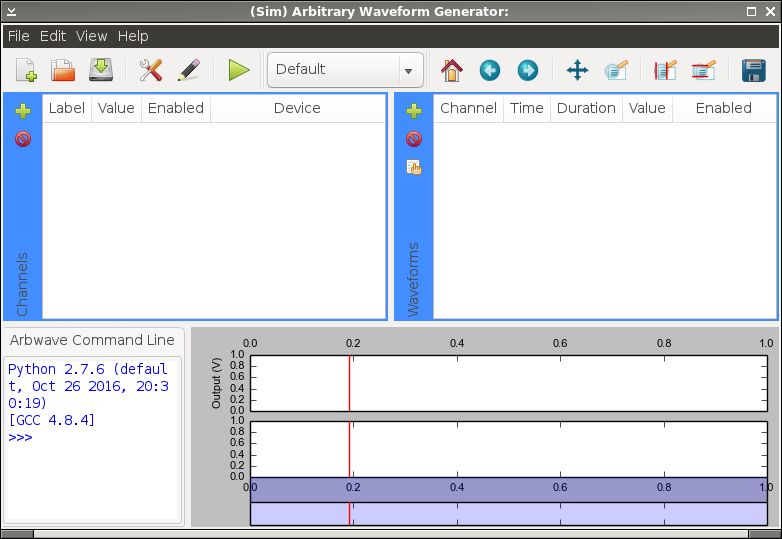
\includegraphics[width=\textwidth]{figures/main-empty}}
  \caption{Main window is empty upon startup}
  \label{fig:quick:main-empty}
\end{figure}



\section{Starting Arbwave}
As discussed in Sec.~\ref{sec:quick:exec} of Chap.~\ref{chap:quickstart},
starting Arbwave is relatively simple using the \verb|run.py| script.
When you first start up Arbwave, you will see an unconfigured instance with a
window that looks like Fig.~\ref{fig:quick:main-empty}.

\subsection{Configuring}
After starting Arbwave, it is necessary to configure devices and signals,
assign channel information, and define waveforms for output.  This should
generally be done following this outline:
%
\begin{enumerate}
  \item Configure Devices (Chap.~\ref{chap:devcfg})

    \begin{enumerate}
      \item Define Connections to Remote Devices
           (Optional--Sec.~\ref{sec:devcfg:conn})

      \item Define Clocks (Sec.~\ref{sec:devcfg:clocks})

      \item Define Signal Routes (Sec.~\ref{sec:devcfg:routes})

      \item Configure Devices (Sec.~\ref{sec:devcfg:devices})
        \begin{itemize}
          \item Define Clock Sources for Devices (Sec.~\ref{sec:devcfg:clksrc})
        \end{itemize}

    \end{enumerate}
  \item Configure Channels
    \begin{enumerate}
      \item Channel Name
        The channel name should be used to very briefly describe the use of the
        particular physical output channel.  For example, for a digital output
        being used to trigger a camera, an appropriate channel name would be
        \textbf{Camera Trigger}.  \textbf{Channel Name} \textit{must} be unique with respect
        to all other enabled channels.
      \item Specifying Device
        The channel device selection describes the underlying hardware device
        and channel on that device that will be bound as the given
        \textbf{Channel Name}.  At most one channel should be bound to an
        underlying hardware output channel for all enabled channels.

      \item Defining Scaling and Units

      \item Static Values
      \item Enabling
    \end{enumerate}
  \item Build Waveforms
    \begin{enumerate}
      \item Define Groups and Waveform Elements
    \end{enumerate}
  \item Execute Waveform
\end{enumerate}
%
Chaps.~\ref{chap:devcfg}--\ref{chap:iterating} give greater detail for the
various steps outlined here.


\subsection{Device Naming Conventions/Styles}\label{sec:op-overview:naming}
Throughout the configuration process, one frequently interact with strings that
represent various devices and signals.  Generally, these devices, signals, and
channels are identified by a type of path, similar to a UNIX file path.

Each device, output channel (analog, digital, timing), or other device item is
uniquely identified by a path that also indicates is logical connections.  For
example, the National Instruments driver path begins with `ni' and subsequent
devices served by this driver should be identified by `sub-directories' within
the `ni' path.  For example, analog channels in the `ni' path are denoted like:
%
\begin{itemize}
  \item ni/Dev1/ao0
  \item ni/Dev1/ao1
  \item ni/Dev2/ao0
  \item ni/Dev2/ao1
\end{itemize}
%
In this example, ni/Dev1/ao is a device that also includes at least channels 0
and 1.  In this example, it is also clear that each device driver must define
its own unique root path identifier, i.e. `ni' for National Instruments, `vp'
for Viewpoint, `uei' for United Electronic Industries, and so forth.
Currently assigned prefixes are shown in Tab.~\ref{tab:prefixes}.

\begin{table}[h!]
  \begin{center}
    \begin{tabular}{|lR{8cm}|}
      \hline
      PREFIX & Backend Driver \\
      \hline
      \hline
      ni     & National Instruments \\
      vp     & Viewpoint \\
      comedi & Comedi \\
      gxt    & Marvin Test GxFpga using AFRL firmware (verified with GX3500) \\
      bbb    & BeagleBone Black (with AFRL firmware/hardware) \\
      \hline
    \end{tabular}
      \caption[Prefixes for device drivers]{\label{tab:prefixes}
        Currently assigned prefixes of various device driver connections
        implemented in Arbwave.
      }
  \end{center}
\end{table}


Common paths should use the same name regardless of which device they are on.
For example, the backplane trigger lines have been given these names (whether
they are being provided by a PXI chassis or a RTSI bus connection):
\begin{itemize}
  \item TRIG/0
  \item TRIG/1
  \item TRIG/2
  \item TRIG/3
  \item TRIG/4
  \item TRIG/5
  \item TRIG/6
\end{itemize}

External, i.e. manual cable connections should be prefixed with `External'.  For
example, if a cable goes from vp/Dev0/A/0 to ni/Dev1/PFI0, there will be two
routing configurations given in the program denoted by:
\begin{itemize}
  \item vp/Dev0/A/0  $\rightarrow$  External/cable0
  \item ni/Dev1/PFI0 $\rightarrow$  External/cable0
\end{itemize}
where the connecting cable has been given the arbitrary, but necessarily
consistent, name of `cable0'.


Connections to remote devices are possible and managed by the
Configure$\rightarrow$Connections tab.  On this tab, a user specifies an alias for a
connection as well as the host name for the connection.
For all connections, nearly all paths will be prefixed by a
representation of the remote host or device.  For example, if a remote system is
identified by the word ``pxi0'', all paths from the corresponding devices of the
remote system will be prefixed by ``pxi0:''.  For example, `ni/Dev1/ao0' would become
`pxi0:ni/Dev1/ao0'.  A user can also specify a default host.  In this case, any
path that does not have the proper ``host:'' prefix will be interpreted to mean
the default connection.
\textbf{NOTE:} The exception to this renaming will be any path that begins with ``External'' as
these are already fairly independent of any device.

The following settings are the default configuration
for connections:
( prefix=`local', host=`localhost', default=True )


\subsection{Commandline Parameters}\label{sec:overview:cmdline}
Arbwave allows various options to be specified on the commandline that alter
Arbwave operation.  The current valid commandline options can also be queried
using the \verb|--help| commandline parameter.  Doing so yields an output such
as:
\begin{verbatim}
usage: arbwave [-h] [--version] [--simulated] [--dataviewer]
               [--log-level {INFO,ALL,WARN,ERROR,DEBUG,FATAL}] [--service]
               [--ipython]
               [--disable {gx3500_dio,bbb,comedi,nidaqmx,viewpoint,external}]
               [--pyro-ns NAMESERVER[:PORT]] [--profile PROFILE]
               [--profile-show PROFILE] [--profile-sort PROFILE_SORT]
               [--profile-n PROFILE_N]
               [filename]

positional arguments:
  filename              configuration file

optional arguments:
  -h, --help            show this help message and exit
  --version             show program's version number and exit
  --simulated           Use simulated hardware
  --dataviewer          Start only the data viewer
  --log-level {INFO,ALL,WARN,ERROR,DEBUG,FATAL}
  --service             Run headless backend service
  --ipython             Attempt to use ipython as embedded shell
  --disable {gx3500_dio,bbb,comedi,nidaqmx,viewpoint,external}
                        Disable specific driver
  --pyro-ns NAMESERVER[:PORT]
                        Specify Pyro nameserver address (in case it cannot be
                        reached by UDP broadcasts). This option will only
                        affect those backends that use the Pyro Nameserver.
                        The default behavior will be to use a broadcast search
                        to find the Pyro Nameserver (which only works if it is
                        on the same subnet).
  --profile PROFILE     Run this script under the observation of a profiler,
                        writing out to the given file. In order to show
                        results, one can use the --profile-show,--profile-sort
                        options. Perhaps an even better way to visualize the
                        profliing results is to use kcachegrind: first convert
                        the results file from this profile to calltree format
                        by using: "hotshot2calltree file.prof > file.calltree"
  --profile-show PROFILE
                        Calculate the results of a previous profile and show
                        the top PROFILE_N worst offenders
  --profile-sort PROFILE_SORT
                        Specify the columns to sort by [Default: time, calls].
                        All possible columns are: cumulative, module, ncalls,
                        pcalls, file, line, name, calls, stdname, nfl,
                        filename, cumtime, time, tottime
  --profile-n PROFILE_N
                        Specify the number of top offenders to show when
                        showing profile results [Default: 20]
\end{verbatim}
